\section{\RU{Касательно сжимания сетевого траффика в клиенте SAP}\EN{About SAP client network traffic compression}}
\label{sec:SAPGUI}

\newcommand{\TDWNC}{TDW\_NOCOMPRESS\xspace}

\RU{(Трассировка связи между переменной окружения \TDWNC{} SAPGUI\footnote{GUI-клиент от SAP}
до \q{назойливого всплывающего окна} и самой функции сжатия данных.)}
\EN{(Tracing the connection between the \TDWNC{} SAPGUI\footnote{SAP GUI client} environment variable and 
the pesky nagging pop-up window and the actual data compression routine.)}

\RU{Известно, что сетевой траффик между SAPGUI и SAP по умолчанию не шифруется, а сжимается} 
\EN{It is known that the network traffic between SAPGUI and SAP is not encrypted by default, but compressed}
(\RU{читайте}\EN{see} \RU{здесь}\EN{here}\footnote{\url{http://go.yurichev.com/17221}} 
\AndENRU 
\RU{здесь}\EN{here}\footnote{\href{http://go.yurichev.com/17225}{blog.yurichev.com}}). 

\RU{Известно также что если установить переменную окружения \IT{\TDWNC} в 1, можно выключить сжатие сетевых пакетов.}
\EN{It is also known that by setting the environment variable \IT{\TDWNC} to 1, it is possible to turn the network packet compression off.}

\RU{Но вы увидите окно, которое нельзя будет закрыть}
\EN{But you will see a nagging pop-up window that cannot be closed}:

\begin{figure}[H]
\centering
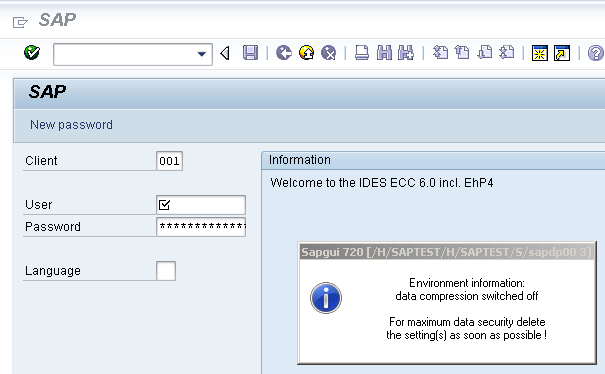
\includegraphics[scale=\FigScale]{examples/SAP/sapgui/sapgui720.png}
\caption{\RU{Скриншот}\EN{Screenshot}}
\end{figure}

\RU{Посмотрим, сможем ли мы как-то убрать это окно}
\EN{Let's see if we can remove the window somehow}.

\RU{Но в начале давайте посмотрим, что мы уже знаем}\EN{But before this, let's see what we already know}.
\RU{Первое: мы знаем, что переменна окружения \IT{\TDWNC} проверяется где-то внутри клиента SAPGUI.}
\EN{First: we know that the environment variable \IT{\TDWNC} is checked somewhere inside the SAPGUI client.}
\RU{Второе: строка вроде \q{data compression switched off} также должна где-то присутствовать.}
\EN{Second: a string like \q{data compression switched off} must be present somewhere in it.}
\newcommand{\FNURLFAR}{\footnote{\url{http://go.yurichev.com/17347}}}
\RU{При помощи файлового менеджера FAR\FNURLFAR мы можем найти обе эти строки в файле SAPguilib.dll.}
\EN{With the help of the FAR file manager\FNURLFAR we can found that both of these strings are stored in the SAPguilib.dll file.}

\RU{Так что давайте откроем файл SAPguilib.dll в \IDA и поищем там строку \IT{\q{\TDWNC}}.
Да, она присутствует и имеется только одна ссылка на эту строку.}
\EN{So let's open SAPguilib.dll in \IDA and search for the \IT{\q{\TDWNC}} string. 
Yes, it is present and there is only one reference to it.}

\RU{Мы увидим такой фрагмент кода
(все смещения верны для версии SAPGUI 720 win32, SAPguilib.dll версия файла 7200,1,0,9009)}
\EN{We see the following fragment of code 
(all file offsets are valid for SAPGUI 720 win32, SAPguilib.dll file version 7200,1,0,9009)}:

\begin{lstlisting}
.text:6440D51B                 lea     eax, [ebp+2108h+var_211C]
.text:6440D51E                 push    eax             ; int
.text:6440D51F                 push    offset aTdw_nocompress ; "TDW_NOCOMPRESS"
.text:6440D524                 mov     byte ptr [edi+15h], 0
.text:6440D528                 call    chk_env
.text:6440D52D                 pop     ecx
.text:6440D52E                 pop     ecx
.text:6440D52F                 push    offset byte_64443AF8
.text:6440D534                 lea     ecx, [ebp+2108h+var_211C]

; demangled name: int ATL::CStringT::Compare(char const *)const
.text:6440D537                 call    ds:mfc90_1603
.text:6440D53D                 test    eax, eax
.text:6440D53F                 jz      short loc_6440D55A
.text:6440D541                 lea     ecx, [ebp+2108h+var_211C]

; demangled name: const char* ATL::CSimpleStringT::operator PCXSTR 
.text:6440D544                 call    ds:mfc90_910
.text:6440D54A                 push    eax             ; Str
.text:6440D54B                 call    ds:atoi
.text:6440D551                 test    eax, eax
.text:6440D553                 setnz   al
.text:6440D556                 pop     ecx
.text:6440D557                 mov     [edi+15h], al
\end{lstlisting}

\index{\CStandardLibrary!atoi()}
\RU{Строка возвращаемая функцией \TT{chk\_env()} через второй аргумент, обрабатывается далее строковыми
функциями MFC, затем вызывается \TT{atoi()}\footnote{Стандартная функция Си, конвертирующая число в строке в число}.
После этого, число сохраняется в \TT{edi+15h}}
\EN{The string returned by \TT{chk\_env()} via its second argument is then handled by the MFC string functions and then 
\TT{atoi()}\footnote{standard C library function that converts the digits in a string to a number} is called. 
After that, the numerical value is stored in \TT{edi+15h}}.

\RU{Обратите также внимание на функцию \TT{chk\_env} (это мы так назвали её вручную)}%
\EN{Also take a look at the \TT{chk\_env()} function (we gave this name to it manually)}:

\begin{lstlisting}
.text:64413F20 ; int __cdecl chk_env(char *VarName, int)
.text:64413F20 chk_env         proc near
.text:64413F20
.text:64413F20 DstSize         = dword ptr -0Ch
.text:64413F20 var_8           = dword ptr -8
.text:64413F20 DstBuf          = dword ptr -4
.text:64413F20 VarName         = dword ptr  8
.text:64413F20 arg_4           = dword ptr  0Ch
.text:64413F20
.text:64413F20                 push    ebp
.text:64413F21                 mov     ebp, esp
.text:64413F23                 sub     esp, 0Ch
.text:64413F26                 mov     [ebp+DstSize], 0
.text:64413F2D                 mov     [ebp+DstBuf], 0
.text:64413F34                 push    offset unk_6444C88C
.text:64413F39                 mov     ecx, [ebp+arg_4]

; (demangled name) ATL::CStringT::operator=(char const *)
.text:64413F3C                 call    ds:mfc90_820 
.text:64413F42                 mov     eax, [ebp+VarName]
.text:64413F45                 push    eax             ; VarName
.text:64413F46                 mov     ecx, [ebp+DstSize]
.text:64413F49                 push    ecx             ; DstSize
.text:64413F4A                 mov     edx, [ebp+DstBuf]
.text:64413F4D                 push    edx             ; DstBuf
.text:64413F4E                 lea     eax, [ebp+DstSize]
.text:64413F51                 push    eax             ; ReturnSize
.text:64413F52                 call    ds:getenv_s
.text:64413F58                 add     esp, 10h
.text:64413F5B                 mov     [ebp+var_8], eax
.text:64413F5E                 cmp     [ebp+var_8], 0
.text:64413F62                 jz      short loc_64413F68
.text:64413F64                 xor     eax, eax
.text:64413F66                 jmp     short loc_64413FBC
.text:64413F68
.text:64413F68 loc_64413F68:
.text:64413F68                 cmp     [ebp+DstSize], 0
.text:64413F6C                 jnz     short loc_64413F72
.text:64413F6E                 xor     eax, eax
.text:64413F70                 jmp     short loc_64413FBC
.text:64413F72
.text:64413F72 loc_64413F72:
.text:64413F72                 mov     ecx, [ebp+DstSize]
.text:64413F75                 push    ecx
.text:64413F76                 mov     ecx, [ebp+arg_4]

; demangled name: ATL::CSimpleStringT<char, 1>::Preallocate(int)
.text:64413F79                 call    ds:mfc90_2691
.text:64413F7F                 mov     [ebp+DstBuf], eax
.text:64413F82                 mov     edx, [ebp+VarName]
.text:64413F85                 push    edx             ; VarName
.text:64413F86                 mov     eax, [ebp+DstSize]
.text:64413F89                 push    eax             ; DstSize
.text:64413F8A                 mov     ecx, [ebp+DstBuf]
.text:64413F8D                 push    ecx             ; DstBuf
.text:64413F8E                 lea     edx, [ebp+DstSize]
.text:64413F91                 push    edx             ; ReturnSize
.text:64413F92                 call    ds:getenv_s
.text:64413F98                 add     esp, 10h
.text:64413F9B                 mov     [ebp+var_8], eax
.text:64413F9E                 push    0FFFFFFFFh
.text:64413FA0                 mov     ecx, [ebp+arg_4]

; demangled name: ATL::CSimpleStringT::ReleaseBuffer(int)
.text:64413FA3                 call    ds:mfc90_5835
.text:64413FA9                 cmp     [ebp+var_8], 0
.text:64413FAD                 jz      short loc_64413FB3
.text:64413FAF                 xor     eax, eax
.text:64413FB1                 jmp     short loc_64413FBC
.text:64413FB3
.text:64413FB3 loc_64413FB3:
.text:64413FB3                 mov     ecx, [ebp+arg_4]

; demangled name: const char* ATL::CSimpleStringT::operator PCXSTR 
.text:64413FB6                 call    ds:mfc90_910
.text:64413FBC
.text:64413FBC loc_64413FBC:
.text:64413FBC
.text:64413FBC                 mov     esp, ebp
.text:64413FBE                 pop     ebp
.text:64413FBF                 retn
.text:64413FBF chk_env         endp
\end{lstlisting}

\index{\CStandardLibrary!getenv()}
\RU{Да}\EN{Yes}. \EN{The}\RU{Функция} \TT{getenv\_s()}\footnote{\href{http://go.yurichev.com/17250}{MSDN}} 
\RU{это \IT{безопасная} версия функции \TT{getenv()}\footnote{Стандартная функция Си, возвращающая значение переменной окружения} в MSVC}
\EN{function is a Microsoft security-enhanced version of \TT{getenv()}\footnote{Standard C library returning environment variable}}.

\index{MFC}
\RU{Тут также имеются манипуляции со строками при помощи функций из MFC}
\EN{There are also some MFC string manipulations}.

\RU{Множество других переменных окружения также проверяются. Здесь список всех переменных проверяемых SAPGUI 
а также сообщение записываемое им в лог-файл, если переменная включена}\EN{Lots of other environment variables are checked as well. 
Here is a list of all variables that are being checked and what SAPGUI would write to its trace log when logging is turned on}:

\begin{center}
\begin{tabular}{ | l | l | }
\hline                        
DPTRACE                  & ``GUI-OPTION: Trace set to \%d'' \\
TDW\_HEXDUMP             & ``GUI-OPTION: Hexdump enabled'' \\
TDW\_WORKDIR             & ``GUI-OPTION: working directory `\%s\''' \\
TDW\_SPLASHSRCEENOFF     & ``GUI-OPTION: Splash Screen Off'' / ``GUI-OPTION: Splash Screen On'' \\
TDW\_REPLYTIMEOUT        & ``GUI-OPTION: reply timeout \%d milliseconds'' \\
TDW\_PLAYBACKTIMEOUT     & ``GUI-OPTION: PlaybackTimeout  set to \%d milliseconds'' \\ 
TDW\_NOCOMPRESS          & ``GUI-OPTION: no compression read'' \\
TDW\_EXPERT              & ``GUI-OPTION: expert mode'' \\
TDW\_PLAYBACKPROGRESS    & ``GUI-OPTION: PlaybackProgress'' \\
TDW\_PLAYBACKNETTRAFFIC  & ``GUI-OPTION: PlaybackNetTraffic'' \\
TDW\_PLAYLOG             & ``GUI-OPTION: /PlayLog is YES, file \%s'' \\
TDW\_PLAYTIME            & ``GUI-OPTION: /PlayTime set to \%d milliseconds'' \\
TDW\_LOGFILE             & ``GUI-OPTION: TDW\_LOGFILE `\%s\''' \\
TDW\_WAN                 & ``GUI-OPTION: WAN - low speed connection enabled'' \\
TDW\_FULLMENU            & ``GUI-OPTION: FullMenu enabled'' \\
SAP\_CP / SAP\_CODEPAGE  & ``GUI-OPTION: SAP\_CODEPAGE `\%d\''' \\
UPDOWNLOAD\_CP           & ``GUI-OPTION: UPDOWNLOAD\_CP `\%d\''' \\
SNC\_PARTNERNAME         & ``GUI-OPTION: SNC name `\%s\''' \\
SNC\_QOP                 & ``GUI-OPTION: SNC\_QOP `\%s\''' \\
SNC\_LIB                 & ``GUI-OPTION: SNC is set to: \%s'' \\ 
SAPGUI\_INPLACE          & ``GUI-OPTION: environment variable SAPGUI\_INPLACE is on'' \\
\hline  
\end{tabular}
\end{center}

\RU{Настройки для каждой переменной записываются в массив через указатель в регистре \EDI. \EDI выставляется перед вызовом функции}
\EN{The settings for each variable are written in the array via a pointer in the \EDI register.
\EDI is set before the function call}:

\begin{lstlisting}
.text:6440EE00                 lea     edi, [ebp+2884h+var_2884] ; options here like +0x15...
.text:6440EE03                 lea     ecx, [esi+24h]
.text:6440EE06                 call    load_command_line
.text:6440EE0B                 mov     edi, eax
.text:6440EE0D                 xor     ebx, ebx
.text:6440EE0F                 cmp     edi, ebx
.text:6440EE11                 jz      short loc_6440EE42
.text:6440EE13                 push    edi
.text:6440EE14                 push    offset aSapguiStoppedA ; "Sapgui stopped after commandline interp"...
.text:6440EE19                 push    dword_644F93E8
.text:6440EE1F                 call    FEWTraceError
\end{lstlisting}

\RU{А теперь, можем ли мы найти строку \IT{\q{data record mode switched on}}?}\EN{Now, can we find the \IT{\q{data record mode switched on}} string?}
\RU{Да, и есть только одна ссылка на эту строку в функции}
\EN{Yes, and the only reference is in} \\
\TT{CDwsGui::PrepareInfoWindow()}.
\RU{Откуда мы узнали имена классов/методов? Здесь много специальных отладочных вызовов, пишущих в лог-файл вроде}%
\EN{How do we get know the class/method names? There are a lot of special debugging calls that write to the log files, like}:

\begin{lstlisting}
.text:64405160                 push    dword ptr [esi+2854h]
.text:64405166                 push    offset aCdwsguiPrepare ; "\nCDwsGui::PrepareInfoWindow: sapgui env"...
.text:6440516B                 push    dword ptr [esi+2848h]
.text:64405171                 call    dbg
.text:64405176                 add     esp, 0Ch
\end{lstlisting}

\dots \OrENRU:

\begin{lstlisting}
.text:6440237A                 push    eax
.text:6440237B                 push    offset aCclientStart_6 ; "CClient::Start: set shortcut user to '\%"...
.text:64402380                 push    dword ptr [edi+4]
.text:64402383                 call    dbg
.text:64402388                 add     esp, 0Ch
\end{lstlisting}

\RU{Они \IT{очень} полезны}\EN{It is \IT{very} useful}.

\RU{Посмотрим содержимое функции \q{назойливого всплывающего окна}}
\EN{So let's see the contents of this pesky nagging pop-up window's function}:

\begin{lstlisting}
.text:64404F4F CDwsGui__PrepareInfoWindow proc near
.text:64404F4F
.text:64404F4F pvParam         = byte ptr -3Ch
.text:64404F4F var_38          = dword ptr -38h
.text:64404F4F var_34          = dword ptr -34h
.text:64404F4F rc              = tagRECT ptr -2Ch
.text:64404F4F cy              = dword ptr -1Ch
.text:64404F4F h               = dword ptr -18h
.text:64404F4F var_14          = dword ptr -14h
.text:64404F4F var_10          = dword ptr -10h
.text:64404F4F var_4           = dword ptr -4
.text:64404F4F
.text:64404F4F                 push    30h
.text:64404F51                 mov     eax, offset loc_64438E00
.text:64404F56                 call    __EH_prolog3
.text:64404F5B                 mov     esi, ecx        ; ECX is pointer to object
.text:64404F5D                 xor     ebx, ebx
.text:64404F5F                 lea     ecx, [ebp+var_14]
.text:64404F62                 mov     [ebp+var_10], ebx

; demangled name: ATL::CStringT(void)
.text:64404F65                 call    ds:mfc90_316    
.text:64404F6B                 mov     [ebp+var_4], ebx
.text:64404F6E                 lea     edi, [esi+2854h]
.text:64404F74                 push    offset aEnvironmentInf ; "Environment information:\n"
.text:64404F79                 mov     ecx, edi

; demangled name: ATL::CStringT::operator=(char const *)
.text:64404F7B                 call    ds:mfc90_820
.text:64404F81                 cmp     [esi+38h], ebx
.text:64404F84                 mov     ebx, ds:mfc90_2539
.text:64404F8A                 jbe     short loc_64404FA9
.text:64404F8C                 push    dword ptr [esi+34h]
.text:64404F8F                 lea     eax, [ebp+var_14]
.text:64404F92                 push    offset aWorkingDirecto ; "working directory: '\%s'\n"
.text:64404F97                 push    eax

; demangled name: ATL::CStringT::Format(char const *,...)
.text:64404F98                 call    ebx ; mfc90_2539
.text:64404F9A                 add     esp, 0Ch
.text:64404F9D                 lea     eax, [ebp+var_14]
.text:64404FA0                 push    eax
.text:64404FA1                 mov     ecx, edi

; demangled name: ATL::CStringT::operator+=(class ATL::CSimpleStringT<char, 1> const &)
.text:64404FA3                 call    ds:mfc90_941
.text:64404FA9
.text:64404FA9 loc_64404FA9:
.text:64404FA9                 mov     eax, [esi+38h]
.text:64404FAC                 test    eax, eax
.text:64404FAE                 jbe     short loc_64404FD3
.text:64404FB0                 push    eax
.text:64404FB1                 lea     eax, [ebp+var_14]
.text:64404FB4                 push    offset aTraceLevelDAct ; "trace level \%d activated\n"
.text:64404FB9                 push    eax

; demangled name: ATL::CStringT::Format(char const *,...)
.text:64404FBA                 call    ebx ; mfc90_2539
.text:64404FBC                 add     esp, 0Ch
.text:64404FBF                 lea     eax, [ebp+var_14]
.text:64404FC2                 push    eax
.text:64404FC3                 mov     ecx, edi

; demangled name: ATL::CStringT::operator+=(class ATL::CSimpleStringT<char, 1> const &)
.text:64404FC5                 call    ds:mfc90_941
.text:64404FCB                 xor     ebx, ebx
.text:64404FCD                 inc     ebx
.text:64404FCE                 mov     [ebp+var_10], ebx
.text:64404FD1                 jmp     short loc_64404FD6
.text:64404FD3
.text:64404FD3 loc_64404FD3:
.text:64404FD3                 xor     ebx, ebx
.text:64404FD5                 inc     ebx
.text:64404FD6
.text:64404FD6 loc_64404FD6:
.text:64404FD6                 cmp     [esi+38h], ebx
.text:64404FD9                 jbe     short loc_64404FF1
.text:64404FDB                 cmp     dword ptr [esi+2978h], 0
.text:64404FE2                 jz      short loc_64404FF1
.text:64404FE4                 push    offset aHexdumpInTrace ; "hexdump in trace activated\n"
.text:64404FE9                 mov     ecx, edi

; demangled name: ATL::CStringT::operator+=(char const *)
.text:64404FEB                 call    ds:mfc90_945
.text:64404FF1
.text:64404FF1 loc_64404FF1:
.text:64404FF1
.text:64404FF1                 cmp     byte ptr [esi+78h], 0
.text:64404FF5                 jz      short loc_64405007
.text:64404FF7                 push    offset aLoggingActivat ; "logging activated\n"
.text:64404FFC                 mov     ecx, edi

; demangled name: ATL::CStringT::operator+=(char const *)
.text:64404FFE                 call    ds:mfc90_945
.text:64405004                 mov     [ebp+var_10], ebx
.text:64405007
.text:64405007 loc_64405007:
.text:64405007                 cmp     byte ptr [esi+3Dh], 0
.text:6440500B                 jz      short bypass
.text:6440500D                 push    offset aDataCompressio ; "data compression switched off\n"
.text:64405012                 mov     ecx, edi

; demangled name: ATL::CStringT::operator+=(char const *)
.text:64405014                 call    ds:mfc90_945
.text:6440501A                 mov     [ebp+var_10], ebx
.text:6440501D
.text:6440501D bypass:
.text:6440501D                 mov     eax, [esi+20h]
.text:64405020                 test    eax, eax
.text:64405022                 jz      short loc_6440503A
.text:64405024                 cmp     dword ptr [eax+28h], 0
.text:64405028                 jz      short loc_6440503A
.text:6440502A                 push    offset aDataRecordMode ; "data record mode switched on\n"
.text:6440502F                 mov     ecx, edi

; demangled name: ATL::CStringT::operator+=(char const *)
.text:64405031                 call    ds:mfc90_945
.text:64405037                 mov     [ebp+var_10], ebx
.text:6440503A
.text:6440503A loc_6440503A:
.text:6440503A
.text:6440503A                 mov     ecx, edi
.text:6440503C                 cmp     [ebp+var_10], ebx
.text:6440503F                 jnz     loc_64405142
.text:64405045                 push    offset aForMaximumData ; "\nFor maximum data security delete\nthe s"...

; demangled name: ATL::CStringT::operator+=(char const *)
.text:6440504A                 call    ds:mfc90_945
.text:64405050                 xor     edi, edi
.text:64405052                 push    edi             ; fWinIni
.text:64405053                 lea     eax, [ebp+pvParam]
.text:64405056                 push    eax             ; pvParam
.text:64405057                 push    edi             ; uiParam
.text:64405058                 push    30h             ; uiAction
.text:6440505A                 call    ds:SystemParametersInfoA
.text:64405060                 mov     eax, [ebp+var_34]
.text:64405063                 cmp     eax, 1600
.text:64405068                 jle     short loc_64405072
.text:6440506A                 cdq
.text:6440506B                 sub     eax, edx
.text:6440506D                 sar     eax, 1
.text:6440506F                 mov     [ebp+var_34], eax
.text:64405072
.text:64405072 loc_64405072:
.text:64405072                 push    edi             ; hWnd
.text:64405073                 mov     [ebp+cy], 0A0h
.text:6440507A                 call    ds:GetDC
.text:64405080                 mov     [ebp+var_10], eax
.text:64405083                 mov     ebx, 12Ch
.text:64405088                 cmp     eax, edi
.text:6440508A                 jz      loc_64405113
.text:64405090                 push    11h             ; i
.text:64405092                 call    ds:GetStockObject
.text:64405098                 mov     edi, ds:SelectObject
.text:6440509E                 push    eax             ; h
.text:6440509F                 push    [ebp+var_10]    ; hdc
.text:644050A2                 call    edi ; SelectObject
.text:644050A4                 and     [ebp+rc.left], 0
.text:644050A8                 and     [ebp+rc.top], 0
.text:644050AC                 mov     [ebp+h], eax
.text:644050AF                 push    401h            ; format
.text:644050B4                 lea     eax, [ebp+rc]
.text:644050B7                 push    eax             ; lprc
.text:644050B8                 lea     ecx, [esi+2854h]
.text:644050BE                 mov     [ebp+rc.right], ebx
.text:644050C1                 mov     [ebp+rc.bottom], 0B4h

; demangled name: ATL::CSimpleStringT::GetLength(void)
.text:644050C8                 call    ds:mfc90_3178
.text:644050CE                 push    eax             ; cchText
.text:644050CF                 lea     ecx, [esi+2854h]

; demangled name: const char* ATL::CSimpleStringT::operator PCXSTR 
.text:644050D5                 call    ds:mfc90_910
.text:644050DB                 push    eax             ; lpchText
.text:644050DC                 push    [ebp+var_10]    ; hdc
.text:644050DF                 call    ds:DrawTextA
.text:644050E5                 push    4               ; nIndex
.text:644050E7                 call    ds:GetSystemMetrics
.text:644050ED                 mov     ecx, [ebp+rc.bottom]
.text:644050F0                 sub     ecx, [ebp+rc.top]
.text:644050F3                 cmp     [ebp+h], 0
.text:644050F7                 lea     eax, [eax+ecx+28h]
.text:644050FB                 mov     [ebp+cy], eax
.text:644050FE                 jz      short loc_64405108
.text:64405100                 push    [ebp+h]         ; h
.text:64405103                 push    [ebp+var_10]    ; hdc
.text:64405106                 call    edi ; SelectObject
.text:64405108
.text:64405108 loc_64405108:
.text:64405108                 push    [ebp+var_10]    ; hDC
.text:6440510B                 push    0               ; hWnd
.text:6440510D                 call    ds:ReleaseDC
.text:64405113
.text:64405113 loc_64405113:
.text:64405113                 mov     eax, [ebp+var_38]
.text:64405116                 push    80h             ; uFlags
.text:6440511B                 push    [ebp+cy]        ; cy
.text:6440511E                 inc     eax
.text:6440511F                 push    ebx             ; cx
.text:64405120                 push    eax             ; Y
.text:64405121                 mov     eax, [ebp+var_34]
.text:64405124                 add     eax, 0FFFFFED4h
.text:64405129                 cdq
.text:6440512A                 sub     eax, edx
.text:6440512C                 sar     eax, 1
.text:6440512E                 push    eax             ; X
.text:6440512F                 push    0               ; hWndInsertAfter
.text:64405131                 push    dword ptr [esi+285Ch] ; hWnd
.text:64405137                 call    ds:SetWindowPos
.text:6440513D                 xor     ebx, ebx
.text:6440513F                 inc     ebx
.text:64405140                 jmp     short loc_6440514D
.text:64405142
.text:64405142 loc_64405142:
.text:64405142                 push    offset byte_64443AF8

; demangled name: ATL::CStringT::operator=(char const *)
.text:64405147                 call    ds:mfc90_820
.text:6440514D
.text:6440514D loc_6440514D:
.text:6440514D                 cmp     dword_6450B970, ebx
.text:64405153                 jl      short loc_64405188
.text:64405155                 call    sub_6441C910
.text:6440515A                 mov     dword_644F858C, ebx
.text:64405160                 push    dword ptr [esi+2854h]
.text:64405166                 push    offset aCdwsguiPrepare ; "\nCDwsGui::PrepareInfoWindow: sapgui env"...
.text:6440516B                 push    dword ptr [esi+2848h]
.text:64405171                 call    dbg
.text:64405176                 add     esp, 0Ch
.text:64405179                 mov     dword_644F858C, 2
.text:64405183                 call    sub_6441C920
.text:64405188
.text:64405188 loc_64405188:
.text:64405188                 or      [ebp+var_4], 0FFFFFFFFh
.text:6440518C                 lea     ecx, [ebp+var_14]

; demangled name: ATL::CStringT::~CStringT()
.text:6440518F                 call    ds:mfc90_601
.text:64405195                 call    __EH_epilog3
.text:6440519A                 retn
.text:6440519A CDwsGui__PrepareInfoWindow endp
\end{lstlisting}

\RU{\ECX в начале функции содержит в себе указатель на объект (потому что это тип функции thiscall~(\myref{thiscall})).
В нашем случае, класс имеет тип, очевидно, \IT{CDwsGui}. 
В зависимости от включенных опций в объекте, 
разные сообщения добавляются к итоговому сообщению.}
\EN{At the start of the function \ECX contains a pointer to the object (since it is a thiscall~(\myref{thiscall})-type of function).
In our case, the object obviously has class type of \IT{CDwsGui}. 
Depending on the option turned on in the object, a specific message part is to be concatenated with the resulting message.}

\RU{Если переменная по адресу \TT{this+0x3D} не ноль, компрессия сетевых пакетов будет выключена}
\EN{If the value at address \TT{this+0x3D} is not zero, the compression is off}:

\begin{lstlisting}
.text:64405007 loc_64405007:
.text:64405007                 cmp     byte ptr [esi+3Dh], 0
.text:6440500B                 jz      short bypass
.text:6440500D                 push    offset aDataCompressio ; "data compression switched off\n"
.text:64405012                 mov     ecx, edi

; demangled name: ATL::CStringT::operator+=(char const *)
.text:64405014                 call    ds:mfc90_945
.text:6440501A                 mov     [ebp+var_10], ebx
.text:6440501D
.text:6440501D bypass:
\end{lstlisting}

\RU{Интересно, что в итоге, состояние переменной \IT{var\_10} определяет, будет ли показано сообщение вообще}
\EN{It is interesting that finally the \IT{var\_10} variable state defines whether the message is to be shown at all}:

\lstinputlisting{\RU{examples/SAP/sapgui/1ru.lst}\EN{examples/SAP/sapgui/1en.lst}}

\RU{Давайте проверим нашу теорию на практике}\EN{Let's check our theory on practice}.

\JNZ \RU{в этой строке}\EN{at this line} \dots

\lstinputlisting{\RU{examples/SAP/sapgui/2ru.lst}\EN{examples/SAP/sapgui/2en.lst}}

\dots \RU{заменим просто на \JMP и получим SAPGUI работающим без этого назойливого всплывающего окна!}
\EN{replace it with just \JMP, and we get SAPGUI working without the pesky nagging pop-up window appearing!}

\RU{Копнем немного глубже и проследим связь между смещением 0x15 в \TT{load\_command\_line()}
(Это мы дали имя этой функции) и переменной \TT{this+0x3D} в \IT{CDwsGui::PrepareInfoWindow}. 
Уверены ли мы что это одна и та же переменная?}
\EN{Now let's dig deeper and find a connection between the $0x15$ offset in the \TT{load\_command\_line()} 
(we gave it this name) function and the \TT{this+0x3D} variable in \IT{CDwsGui::PrepareInfoWindow}. 
Are we sure the value is the same?}

\RU{Начинаем искать все места где в коде используется константа \TT{0x15}.
Для таких небольших программ как SAPGUI, это иногда срабатывает. Вот первое что находим:}
\EN{We are starting to search for all occurrences of the \TT{0x15} value in code. 
For a small programs like SAPGUI, it sometimes works. Here is the first occurrence we've got:}

\begin{lstlisting}
.text:64404C19 sub_64404C19    proc near
.text:64404C19
.text:64404C19 arg_0           = dword ptr  4
.text:64404C19
.text:64404C19                 push    ebx
.text:64404C1A                 push    ebp
.text:64404C1B                 push    esi
.text:64404C1C                 push    edi
.text:64404C1D                 mov     edi, [esp+10h+arg_0]
.text:64404C21                 mov     eax, [edi]
.text:64404C23                 mov     esi, ecx ; ESI/ECX are pointers to some unknown object.
.text:64404C25                 mov     [esi], eax
.text:64404C27                 mov     eax, [edi+4]
.text:64404C2A                 mov     [esi+4], eax
.text:64404C2D                 mov     eax, [edi+8]
.text:64404C30                 mov     [esi+8], eax
.text:64404C33                 lea     eax, [edi+0Ch]
.text:64404C36                 push    eax
.text:64404C37                 lea     ecx, [esi+0Ch]

; demangled name:  ATL::CStringT::operator=(class ATL::CStringT ... &)
.text:64404C3A                 call    ds:mfc90_817 
.text:64404C40                 mov     eax, [edi+10h]
.text:64404C43                 mov     [esi+10h], eax
.text:64404C46                 mov     al, [edi+14h]
.text:64404C49                 mov     [esi+14h], al
.text:64404C4C                 mov     al, [edi+15h] ; copy byte from 0x15 offset
.text:64404C4F                 mov     [esi+15h], al ; to 0x15 offset in CDwsGui object
\end{lstlisting}

\RU{Эта функция вызывается из функции с названием \IT{CDwsGui::CopyOptions}! И снова спасибо отладочной информации.}
\EN{The function was called from the function named \IT{CDwsGui::CopyOptions}! And thanks again for debugging information.}

\RU{Но настоящий ответ находится в функции}\EN{But the real answer is in} \IT{CDwsGui::Init()}:

\begin{lstlisting}
.text:6440B0BF loc_6440B0BF:
.text:6440B0BF                 mov     eax, [ebp+arg_0]
.text:6440B0C2                 push    [ebp+arg_4]
.text:6440B0C5                 mov     [esi+2844h], eax
.text:6440B0CB                 lea     eax, [esi+28h] ; ESI is pointer to CDwsGui object
.text:6440B0CE                 push    eax
.text:6440B0CF                 call    CDwsGui__CopyOptions
\end{lstlisting}

\RU{Теперь ясно: массив заполняемый в \TT{load\_command\_line()} на самом деле расположен в классе \IT{CDwsGui} но по адресу
\TT{this+0x28}. 0x15 + 0x28 это 0x3D. ОК, мы нашли место, куда наша переменная копируется.}
\EN{Finally, we understand: the array filled in the \TT{load\_command\_line()} function is actually placed in the \IT{CDwsGui} class, 
but at address \TT{this+0x28}. 0x15 + 0x28 is exactly 0x3D. OK, we found the point where the value is copied to.}

\RU{Посмотрим также и другие места, где используется смещение 0x3D.
Одно из таких мест находится в функции \IT{CDwsGui::SapguiRun} (и снова спасибо отладочным вызовам):}
\EN{Let's also find the rest of the places where the 0x3D offset is used. 
Here is one of them in the \IT{CDwsGui::SapguiRun} function (again, thanks to the debugging calls):}

\begin{lstlisting}
.text:64409D58                 cmp     [esi+3Dh], bl   ; ESI is pointer to CDwsGui object
.text:64409D5B                 lea     ecx, [esi+2B8h]
.text:64409D61                 setz    al
.text:64409D64                 push    eax             ; arg_10 of CConnectionContext::CreateNetwork
.text:64409D65                 push    dword ptr [esi+64h]

; demangled name: const char* ATL::CSimpleStringT::operator PCXSTR 
.text:64409D68                 call    ds:mfc90_910
.text:64409D68                                         ; no arguments
.text:64409D6E                 push    eax
.text:64409D6F                 lea     ecx, [esi+2BCh]

; demangled name: const char* ATL::CSimpleStringT::operator PCXSTR 
.text:64409D75                 call    ds:mfc90_910
.text:64409D75                                         ; no arguments
.text:64409D7B                 push    eax
.text:64409D7C                 push    esi
.text:64409D7D                 lea     ecx, [esi+8]
.text:64409D80                 call    CConnectionContext__CreateNetwork
\end{lstlisting}

\RU{Проверим нашу идею. Заменяем \TT{setz al} здесь на \TT{xor eax, eax / nop}, убираем переменную окружения 
\TDWNC и запускаем SAPGUI. Ух! Назойливого окна больше нет (как и ожидалось: ведь переменной окружении также
нет), но в Wireshark мы видим, что сетевые пакеты больше не сжимаются!
Очевидно, это то самое место где флаг отражающий сжатие пакетов выставляется в объекте \TT{CConnectionContext}.}
\EN{Let's check our findings. Replace the \TT{setz al} here with the \TT{xor eax, eax / nop} instructions,
clear the \TDWNC 
environment variable and run SAPGUI. Wow! There pesky nagging window is no more (just as expected, 
because the variable is not set) but in Wireshark we can see that the network packets are not compressed anymore! 
Obviously, this is the point where the compression flag is to be set in the \IT{CConnectionContext} object.}

\RU{Так что, флаг сжатия передается в пятом аргументе функции \IT{CConnectionContext::CreateNetwork}. 
Внутри этой функции, вызывается еще одна:}
\EN{So, the compression flag is passed in the 5th argument of \IT{CConnectionContext::CreateNetwork}. 
Inside the function, another one is called:}

\begin{lstlisting}
...
.text:64403476                 push    [ebp+compression]
.text:64403479                 push    [ebp+arg_C]
.text:6440347C                 push    [ebp+arg_8]
.text:6440347F                 push    [ebp+arg_4]
.text:64403482                 push    [ebp+arg_0]
.text:64403485                 call    CNetwork__CNetwork
\end{lstlisting}

\RU{Флаг отвечающий за сжатие здесь передается в пятом аргументе для конструктора \IT{CNetwork::CNetwork}.}
\EN{The compression flag is passed here in the 5th argument to the \IT{CNetwork::CNetwork} constructor.}

\RU{И вот как конструктор \IT{CNetwork} выставляет некоторые флаги в объекте \IT{CNetwork} в соответствии с пятым аргументом \IT{и}
еще какую-то переменную, возможно, также отвечающую за сжатие сетевых пакетов.}
\EN{And here is how the \IT{CNetwork} constructor sets the flag in the \IT{CNetwork} object according to its 5th argument \IT{and}
another variable which probably could also affect network packets compression.}

\begin{lstlisting}
.text:64411DF1                 cmp     [ebp+compression], esi
.text:64411DF7                 jz      short set_EAX_to_0
.text:64411DF9                 mov     al, [ebx+78h]   ; another value may affect compression?
.text:64411DFC                 cmp     al, '3'
.text:64411DFE                 jz      short set_EAX_to_1
.text:64411E00                 cmp     al, '4'
.text:64411E02                 jnz     short set_EAX_to_0
.text:64411E04
.text:64411E04 set_EAX_to_1:
.text:64411E04                 xor     eax, eax
.text:64411E06                 inc     eax             ; EAX -> 1
.text:64411E07                 jmp     short loc_64411E0B
.text:64411E09
.text:64411E09 set_EAX_to_0:
.text:64411E09
.text:64411E09                 xor     eax, eax        ; EAX -> 0
.text:64411E0B
.text:64411E0B loc_64411E0B:
.text:64411E0B                 mov     [ebx+3A4h], eax ; EBX is pointer to CNetwork object
\end{lstlisting}

\RU{Теперь мы знаем, что флаг отражающий сжатие данных сохраняется в классе \IT{CNetwork} по адресу \IT{this+0x3A4}.}
\EN{At this point we know the compression flag is stored in the \IT{CNetwork} class at address \IT{this+0x3A4}.}

\RU{Поищем теперь значение \TT{0x3A4} в SAPguilib.dll. Находим второе упоминание этого значения в функции
\IT{CDwsGui::OnClientMessageWrite} (бесконечная благодарность отладочной информации):}
\EN{Now let's dig through SAPguilib.dll for the \TT{0x3A4} value. And here is the second occurrence in 
\IT{CDwsGui::OnClientMessageWrite} (endless thanks for the debugging information):}

\begin{lstlisting}
.text:64406F76 loc_64406F76:
.text:64406F76                 mov     ecx, [ebp+7728h+var_7794]
.text:64406F79                 cmp     dword ptr [ecx+3A4h], 1
.text:64406F80                 jnz     compression_flag_is_zero
.text:64406F86                 mov     byte ptr [ebx+7], 1
.text:64406F8A                 mov     eax, [esi+18h]
.text:64406F8D                 mov     ecx, eax
.text:64406F8F                 test    eax, eax
.text:64406F91                 ja      short loc_64406FFF
.text:64406F93                 mov     ecx, [esi+14h]
.text:64406F96                 mov     eax, [esi+20h]
.text:64406F99
.text:64406F99 loc_64406F99:
.text:64406F99                 push    dword ptr [edi+2868h] ; int
.text:64406F9F                 lea     edx, [ebp+7728h+var_77A4]
.text:64406FA2                 push    edx             ; int
.text:64406FA3                 push    30000           ; int
.text:64406FA8                 lea     edx, [ebp+7728h+Dst]
.text:64406FAB                 push    edx             ; Dst
.text:64406FAC                 push    ecx             ; int
.text:64406FAD                 push    eax             ; Src
.text:64406FAE                 push    dword ptr [edi+28C0h] ; int
.text:64406FB4                 call    sub_644055C5       ; actual compression routine
.text:64406FB9                 add     esp, 1Ch
.text:64406FBC                 cmp     eax, 0FFFFFFF6h
.text:64406FBF                 jz      short loc_64407004
.text:64406FC1                 cmp     eax, 1
.text:64406FC4                 jz      loc_6440708C
.text:64406FCA                 cmp     eax, 2
.text:64406FCD                 jz      short loc_64407004
.text:64406FCF                 push    eax
.text:64406FD0                 push    offset aCompressionErr ; "compression error [rc = \%d]- program wi"...
.text:64406FD5                 push    offset aGui_err_compre ; "GUI_ERR_COMPRESS"
.text:64406FDA                 push    dword ptr [edi+28D0h]
.text:64406FE0                 call    SapPcTxtRead
\end{lstlisting}

\RU{Заглянем в функцию \IT{sub\_644055C5}. Всё что в ней мы находим это вызов memcpy() и еще какую-то функцию, названную
\IDA \IT{sub\_64417440}.}
\EN{Let's take a look in \IT{sub\_644055C5}. In it we can only see the call to memcpy() and another function named 
(by \IDA) \IT{sub\_64417440}.}

\RU{И теперь заглянем в \IT{sub\_64417440}. Увидим там:}
\EN{And, let's take a look inside \IT{sub\_64417440}. What we see is:}

\begin{lstlisting}
.text:6441747C                 push    offset aErrorCsrcompre ; "\nERROR: CsRCompress: invalid handle"
.text:64417481                 call    eax ; dword_644F94C8
.text:64417483                 add     esp, 4
\end{lstlisting}

Voilà! \RU{Мы находим функцию которая собственно и сжимает сетевые пакеты.}\EN{We've found the function that actually compresses the data.}
\RU{Как я уже разобрался}\EN{As I've shown in past}
\footnote{\url{http://go.yurichev.com/17312}},
\RU{эта функция используется в SAP и в опен-сорсном проекте MaxDB.
Так что эта функция доступна в виде исходников.}
\EN{this function is used in SAP and also the open-source MaxDB project. 
So it is available in source form.}

\RU{Последняя проверка:}\EN{Doing the last check here:}

\begin{lstlisting}
.text:64406F79                 cmp     dword ptr [ecx+3A4h], 1
.text:64406F80                 jnz     compression_flag_is_zero
\end{lstlisting}

\RU{Заменим \JNZ на безусловный переход \JMP. Уберем переменную окружения \TDWNC. Вуаля!}
\EN{Replace \JNZ here for an unconditional \JMP. Remove the environment variable \TDWNC. Voilà!}
\RU{В Wireshark мы видим, что сетевые пакеты, исходящие от клиента, не сжаты. Ответы сервера, впрочем, сжаты.}
\EN{In Wireshark we see that the client messages are not compressed. The server responses, however, are compressed.}

\RU{Так что мы нашли связь между переменной окружения и местом где функция сжатия данных вызывается, а также
может быть отключена.}
\EN{So we found exact connection between the environment variable and the point where data compression 
routine can be called or bypassed.}

